%%%%%%%% ICML 2025 EXAMPLE LATEX SUBMISSION FILE %%%%%%%%%%%%%%%%%

\documentclass{article}

% Recommended, but optional, packages for figures and better typesetting:
\usepackage{microtype}
\usepackage{graphicx}
\usepackage{subfigure}
\usepackage{booktabs} % for professional tables

% hyperref makes hyperlinks in the resulting PDF.
% If your build breaks (sometimes temporarily if a hyperlink spans a page)
% please comment out the following usepackage line and replace
% \usepackage{icml2025} with \usepackage[nohyperref]{icml2025} above.
\usepackage{hyperref}


% Attempt to make hyperref and algorithmic work together better:
\newcommand{\theHalgorithm}{\arabic{algorithm}}

% Use the following line for the initial blind version submitted for review:
\usepackage{icml2025}

% If accepted, instead use the following line for the camera-ready submission:
% \usepackage[accepted]{icml2025}

% For theorems and such
\usepackage{amsmath}
\usepackage{amssymb}
\usepackage{mathtools}
\usepackage{amsthm}

% if you use cleveref..
\usepackage[capitalize,noabbrev]{cleveref}

% Give wide floats more room so the qualitative figure places near its
% discussion rather than being deferred to the appendix.
\renewcommand{\topfraction}{0.9}
\renewcommand{\bottomfraction}{0.8}
\renewcommand{\textfraction}{0.07}
\renewcommand{\floatpagefraction}{0.7}
\setcounter{topnumber}{3}
\setcounter{totalnumber}{4}

%%%%%%%%%%%%%%%%%%%%%%%%%%%%%%%%
% THEOREMS
%%%%%%%%%%%%%%%%%%%%%%%%%%%%%%%%
\theoremstyle{plain}
\newtheorem{theorem}{Theorem}[section]
\newtheorem{proposition}[theorem]{Proposition}
\newtheorem{lemma}[theorem]{Lemma}
\newtheorem{corollary}[theorem]{Corollary}
\theoremstyle{definition}
\newtheorem{definition}[theorem]{Definition}
\newtheorem{assumption}[theorem]{Assumption}
\theoremstyle{remark}
\newtheorem{remark}[theorem]{Remark}

% Todonotes is useful during development; simply uncomment the next line
%    and comment out the line below the next line to turn off comments
%\usepackage[disable,textsize=tiny]{todonotes}
\usepackage[textsize=tiny]{todonotes}


% The \icmltitle you define below is probably too long as a header.
% Therefore, a short form for the running title is supplied here:
\icmltitlerunning{Supervised Saliency Alignment for Visual Grounding in Vision-Language Models}

\begin{document}

\twocolumn[
\icmltitle{
    Look at This: Supervised Saliency Alignment for Visual Grounding in Vision-Language Models
}

% It is OKAY to include author information, even for blind
% submissions: the style file will automatically remove it for you
% unless you've provided the [accepted] option to the icml2025
% package.

% List of affiliations: The first argument should be a (short)
% identifier you will use later to specify author affiliations
% Academic affiliations should list Department, University, City, Region, Country
% Industry affiliations should list Company, City, Region, Country

% You can specify symbols, otherwise they are numbered in order.
% Ideally, you should not use this facility. Affiliations will be numbered
% in order of appearance and this is the preferred way.
\icmlsetsymbol{equal}{*}

\begin{icmlauthorlist}
\icmlauthor{Alexander Brady}{equal,eth}
\icmlauthor{Tim Eilers}{equal,eth}
\icmlauthor{Mubashara Akhtar}{eth}
\icmlauthor{Sunghwan Hong}{eth}
\icmlauthor{Yifan Hou}{eth}
\icmlauthor{Junling Wang}{eth}
\end{icmlauthorlist}

\icmlaffiliation{eth}{ETH Zürich}
% \icmlaffiliation{yyy}{Department of XXX, University of YYY, Location, Country}
% \icmlaffiliation{comp}{Company Name, Location, Country}
% \icmlaffiliation{sch}{School of ZZZ, Institute of WWW, Location, Country}

\icmlcorrespondingauthor{Alexander Brady}{bradya@ethz.ch}
\icmlcorrespondingauthor{Tim Eilers}{teilers@ethz.ch}

% You may provide any keywords that you
% find helpful for describing your paper; these are used to populate
% the "keywords" metadata in the PDF but will not be shown in the document
\icmlkeywords{Machine Learning, ICML, Vision Language Models, Visual Grounding}

\vskip 0.3in
]

% this must go after the closing bracket ] following \twocolumn[ ...

% This command actually creates the footnote in the first column
% listing the affiliations and the copyright notice.
% The command takes one argument, which is text to display at the start of the footnote.
% The \icmlEqualContribution command is standard text for equal contribution.
% Remove it (just {}) if you do not need this facility.

%\printAffiliationsAndNotice{}  % leave blank if no need to mention equal contribution
\printAffiliationsAndNotice{\icmlEqualContribution} % otherwise use the standard text.

\begin{abstract}
Vision--language models (VLMs) learn rich image--text associations, yet they reason with poorly localized visual attention: the saliency maps induced by their attention are noisy, place mass on irrelevant regions, and only loosely track the objects a token describes. We introduce the \emph{Saliency Alignment Loss}, a training-time auxiliary objective that supervises a VLM's token-conditioned attention with region-level grounding annotations. For each generated token we read out a saliency map over the image patches and minimize its divergence from a target distribution supported on the token's annotated region, jointly with the standard captioning loss. The objective adds no parameters and leaves the architecture untouched, dropping into ordinary fine-tuning pipelines. Fine-tuning LLaVA-1.5-7B on the densely grounded COCONut-PanCap captions for only $200$ steps, we measure alignment intrinsically on held-out images with three metrics---chance-normalized Attention Mass Ratio, pixel-level Average Precision, and Normalized Scanpath Saliency---chosen to sidestep the COCO contamination that pervades public grounding benchmarks. Alignment transforms saliency---mean Attention Mass Ratio rises $4.6{\times}$ and the maps visibly concentrate on the relevant objects---while leaving language quality intact. We trace \emph{where} this adaptation occurs: the language model, not the multimodal projector, absorbs the signal, reaching a reproducible low-rank solution in a small set of grounding-relevant attention heads. We are equally explicit about its limits: the intrinsic gains do not yet transfer to downstream benchmarks, saliency quality and task grounding are dissociated, and alignment withdraws attention from background ``stuff'' the annotations never cover. These findings motivate an in-progress instruction-tuned variant designed to convert sharper attention into better grounding.

\end{abstract}

\section{Introduction}
\label{sec:introduction}
Vision--language models (VLMs) combine a pretrained vision encoder with a large language model and achieve strong performance across a broad range of multimodal tasks. Yet they remain unreliable on tasks that require fine-grained, spatially grounded understanding (counting, referential grounding, and spatial reasoning), where predictions often reflect shortcut correlations and scene-level priors rather than evidence drawn from the queried region~\citep{chenspatial, sengupta2025can}.

A growing body of work locates part of this failure in how VLMs allocate visual attention. The attention from a generated token to the image patches can be read out as a \emph{saliency map}, and the degree to which this map overlaps the relevant object correlates with answer correctness~\citep{chenspatial}. In practice these maps are frequently mislocalized: attention disperses over non-informative regions, image borders, and background, and only a small subset of specialized heads attend in a grounding-relevant way~\citep{kangsee, kang2025your, kim2025interpreting}. Tellingly, \emph{shaping} the attention distribution (suppressing distractor regions) helps more than simply increasing the attention mass on targets~\citep{sengupta2025can}. Attention is thus both a faithful diagnostic of grounding and a promising intervention point.

Existing remedies stop short of supervising this signal directly. Inference-time methods reallocate or mask attention with hand-designed heuristics but never change what the model has learned. Representation-alignment objectives, which regularize a VLM's hidden states toward a pretrained vision encoder~\citep{yurepresentation, yoon2025visual}, do change the model, but their target is a \emph{static}, query-agnostic feature map: it cannot express that a token should attend \emph{here} for \emph{this} prompt. What is missing is a training-time objective that supervises the token-conditioned attention itself against where the evidence actually is.

We close this gap with the \textbf{Saliency Alignment Loss}: an auxiliary objective that, during fine-tuning, pulls each generated token's saliency map toward the image region its referent occupies. Using a densely grounded captioning corpus, COCONut-PanCap~\citep{deng2025coconut}, we attach a target distribution (uniform over the token's annotated mask) to every grounded token and minimize the divergence from the model's saliency through a Kullback--Leibler term added to the usual captioning loss. The objective introduces no new parameters and no architectural change, and because grounding benchmarks are overwhelmingly derived from COCO~\citep{han2024coco} (and therefore overlap our training images), we evaluate alignment \emph{intrinsically}, on held-out images, with three complementary attention-localization metrics.

Fine-tuning LLaVA-1.5-7B for only $200$ steps already reshapes its attention: all three localization metrics improve sharply (mean Attention Mass Ratio $4.6{\times}$) and the maps visibly concentrate on the objects a token names. We then ask \emph{where} this adaptation lives, and find, by parameter-drift analysis, that the language model, not the multimodal projector, absorbs the gradient, reaching a solution that is strikingly reproducible across runs and that preferentially moves a subset of attention heads, echoing the localization-head hypothesis~\citep{kang2025your}. Our most consequential finding, however, is what does \emph{not} change: despite the large intrinsic gains, downstream benchmarks barely move, saliency-map quality and task grounding turn out to be \emph{dissociated} (across configurations even anti-correlated with counting), and the objective withdraws attention from broad background ``stuff'' (snow, sky) the annotations never cover. We therefore present alignment as an effective but double-edged tool, and outline an instruction-tuned variant that ports the objective into the standard LLaVA-1.5 recipe to target the transfer gap.

\paragraph{Contributions.}
\begin{itemize}
    \item We propose the Saliency Alignment Loss, a parameter-free, architecture-agnostic training objective that supervises a VLM's token-conditioned attention with region-level grounding annotations (\Cref{sec:method}), together with an intrinsic, contamination-aware protocol (AMR, AP, NSS) for measuring attention localization on held-out data (\Cref{sec:metrics}).
    \item Our central empirical finding is a \emph{dissociation}: alignment improves the intrinsic metrics by large margins yet leaves downstream benchmarks essentially unchanged, and, across training configurations, attention quality is even anti-correlated with counting accuracy. Sharper attention is not, on its own, better grounding (\Cref{sec:results,sec:analysis}).
    \item We localize \emph{where} the model adapts through parameter-drift analysis: the language model rather than the projector absorbs the signal, identically with or without the projector trainable and reproducibly across runs; and we characterize a background-``stuff'' failure mode and root it in the annotation distribution (\Cref{sec:analysis}).
\end{itemize}


\section{Related Work}
\label{sec:relatedwork}
\textbf{Visual Attention Structure in VLMs.}
A growing body of research examines how vision-language models (VLMs) allocate visual attention in order to assess their visual grounding capabilities. Prior studies show that, although vision tokens often receive limited overall attention, increasing attention mass alone does not improve spatial reasoning performance; instead, the \emph{localization} of attention is the dominant factor~\citep{chenspatial}. In particular, overlap between attention maps and ground-truth object regions strongly correlates with answer correctness, indicating that attention localization encodes meaningful grounding signals rather than serving as a purely interpretative tool.

Further work confirms that VLM attention is frequently mislocalized, with excessive focus on non-informative regions, degrading performance on visual grounding tasks such as counting and spatial reasoning~\citep{kangsee, anwenbin2025mitigating}. Several strategies have been proposed to mitigate this issue, including attention reallocation and masking schemes. Notably, suppressing attention to distractor regions is often more effective than amplifying attention to target regions, highlighting the importance of shaping attention distributions rather than merely increasing their magnitude~\citep{sengupta2025can}.

Finally, attention allocation varies substantially across layers and heads. Rather than being uniformly distributed, grounding-relevant attention is often concentrated in a small subset of specialized heads, which exhibit more accurate localization and improved interpretability~\citep{kang2025your, kim2025interpreting}. These findings suggest that attention mechanisms constitute a promising intervention point for improving visual grounding in VLMs.

\textbf{Supervised Representation Objectives.} 
Several lines of work explore supervised objectives that align internal model representations with external visual signals. Representation alignment (REPA) has proven effective in other generative settings, for example diffusion models, where aligning hidden states with pretrained visual encoders improves both training efficiency and generation quality~\citep{yurepresentation}.

Building on this idea, recent work aligns internal representations of VLMs with those of pretrained vision encoders, leading to improved visual grounding and multimodal reasoning~\citep{yoon2025visual}. However, such approaches operate on static visual features that are independent of the textual prompt and generated tokens, limiting their ability to capture context-dependent grounding behavior.

More closely related to our work, \citet{chefer2022optimizing} propose directly supervising attention maps in unimodal vision transformers using ground-truth region annotations, demonstrating improved robustness and domain generalization. Unlike static feature representations, attention maps in VLMs are inherently prompt- and token-dependent, evolving dynamically during text generation. This property enables context-sensitive visual grounding that cannot be captured by feature-level alignment alone. We build on this insight by extending attention-level supervision to the vision-language setting, aligning token-conditioned attention maps with region-level grounding annotations during generation.

Existing approaches either apply inference-time attention heuristics, or align static visual representations that are independent of the generated text. To our knowledge, no prior work introduces a training-time attention supervision objective that explicitly aligns token-conditioned attention in VLMs with region-level grounding annotations. Our work fills this gap by supervising dynamic attention maps during text generation, enabling context-sensitive visual grounding.

% -\citep{paiss2023teaching} - in CLIP, a counting-contrastive loss is used to align image-text representations, improving counting ability and making more interpretable attention maps. Can we find similar results in VLMs?

\section{Preliminaries}
\label{sec:background}
\textbf{Vision-Language Models (VLMs).} We consider VLMs that pair a Vision Transformer (ViT)~\citep{dosovitskiy2020vit} with an autoregressive text decoder. The ViT encodes an input image $\mathbf{I}$ into a sequence of patch embeddings $\{v_i\}_{i=1}^{N}$, which serve as \emph{patch tokens}. A projection module maps these tokens into the language model's embedding space, where they act as conditioning context. The decoder then predicts tokens $\{w_t\}_{t=1}^{T}$ autoregressively under the standard next-token prediction objective. In LLaVA-1.5-7B, the ViT is a CLIP ViT-L/14 operating at $336{\times}336$ resolution, giving an $N = 24{\times}24 = 576$ patch grid, and the decoder is Vicuna-7B.

\textbf{Saliency Maps.} Because patch tokens and text tokens are processed jointly within the decoder's self-attention layers, each generated token $w_t$ attends to all $N$ patch tokens. We form a saliency map $\mathbf{S}_t$ for $w_t$ by aggregating these token-to-patch attention weights across layers and heads and reshaping the result onto the ViT patch grid, producing a spatial map that highlights the regions most relevant to predicting $w_t$. Throughout, we normalize $\mathbf{S}_t$ to a probability distribution over spatial locations so that maps are comparable across images and tokens. This saliency signal is the quantity our objective supervises (\Cref{sec:method}) and our metrics evaluate (\Cref{sec:experiment}).


\section{Method}
\label{sec:method}
Our objective supervises \emph{where} a VLM attends as it generates text, aligning each token's saliency map with the image region its referent occupies. The idea is simple: when the model emits a word that names an annotated entity, the saliency for that word should land on that entity.

\textbf{Token-level grounding signal.}
We assume training captions carry token-level grounding annotations. For a generated caption token $c_t$ that refers to one or more image segments, let $\mathbf{M}_t \in \{0,1\}^{H \times W}$ be the binary mask covering its annotated region(s). From the model's attention we form the saliency map $\mathbf{S}_t$ over the $N$ patch tokens (\Cref{sec:background}), bilinearly upsample it to the annotation resolution $H \times W$, and apply a spatial softmax so that $\mathbf{S}_t$ is a distribution over pixels, $\sum_{ij}\mathbf{S}_{t,ij}=1$. We supervise only the set $\mathcal{T}$ of \emph{grounded} tokens---those annotated with at least one segment---and leave all other tokens (function words, punctuation) to the language modeling loss alone.

\textbf{Alignment loss.}
We compare $\mathbf{S}_t$ against the target distribution that places probability uniformly over the annotated region,
\begin{equation}
\mathbf{T}_t = \mathbf{M}_t \,/\, |\mathbf{M}_t|,
\end{equation}
and penalize their divergence. Our primary objective uses the Kullback--Leibler divergence,
\begin{equation}
\mathcal{L}_{\text{align}}
= \frac{1}{|\mathcal{T}|} \sum_{t \in \mathcal{T}}
\mathrm{KL}\!\left(\mathbf{T}_t \,\|\, \mathbf{S}_t\right)
= \frac{1}{|\mathcal{T}|} \sum_{t \in \mathcal{T}} \sum_{i,j}
\mathbf{T}_{t,ij} \log \frac{\mathbf{T}_{t,ij}}{\mathbf{S}_{t,ij}} .
\label{eq:align}
\end{equation}
Because the target $\mathbf{T}_t$ is fixed, minimizing $\mathrm{KL}(\mathbf{T}_t \,\|\, \mathbf{S}_t)$ is mass-covering: it drives $\mathbf{S}_t$ to put probability everywhere inside the mask and is heavily penalized wherever the mask is occupied but the saliency is near zero, encouraging the map to cover the \emph{whole} referent rather than collapse onto a single patch. As a point of comparison we also implement a squared-error variant, $\mathcal{L}_{\text{align}}^{\text{MSE}} = \frac{1}{|\mathcal{T}|}\sum_{t}\sum_{ij}(\mathbf{S}_{t,ij}-\mathbf{T}_{t,ij})^2$, and use the KL form by default.

\textbf{Training objective.}
We add the alignment term to the standard captioning cross-entropy,
\begin{equation}
\mathcal{L}_{\text{total}} = \mathcal{L}_{\text{CE}} + \lambda \cdot \mathcal{L}_{\text{align}},
\label{eq:total}
\end{equation}
where $\lambda$ trades off fluency against grounding. The term introduces no new parameters and no architectural change, so it drops into a standard VLM fine-tuning pipeline. The vision encoder is kept frozen throughout; which of the remaining components actually absorbs the alignment gradient---the multimodal projector, the language model, or both---is a design choice we treat as an ablation (\Cref{sec:experiment}) and dissect mechanistically in \Cref{sec:analysis}.


\section{Experimental Setup}
\label{sec:experiment}
\subsection{Dataset and grounding signal}
We fine-tune on COCONut-PanCap~\citep{deng2025coconut}, which pairs COCO images~\citep{lin2015microsoftcococommonobjects} with high-quality panoptic masks and human-verified, detailed captions. Crucially, each caption is \emph{grounded}: mentioned entities are tagged with the panoptic segment(s) they refer to, in the form \texttt{<id: text>} (or \texttt{<$id_1,\dots,id_k$: text>} for groups). We parse these tags to (i) recover the clean caption shown to the model and (ii) assign every caption token the segment id(s) it references; the per-token mask $\mathbf{M}_t$ of \Cref{sec:method} is then the union of the referenced segments in the panoptic mask. Relative to grounded-caption corpora such as GranD~\citep{rasheed2024glammpixelgroundinglarge} or PNG~\citep{gonzalez2021panopticnarrativegrounding}, COCONut-PanCap provides substantially denser annotations, yielding more supervised tokens per image. We use a deterministic split that holds out the last $10{,}000$ annotated images for validation and trains on the remainder; the same split is reused at evaluation so all reported metrics are computed on images the model never saw.

\subsection{Model and training}
We fine-tune LLaVA-1.5-7B with the objective of \Cref{eq:total} at $\lambda = 0.5$, using the model's own prompt template with the instruction \emph{``Describe the image in detail.''} and the clean caption as the target. The vision encoder is always frozen. Optimization uses AdamW (learning rate $2\times10^{-5}$), bf16-mixed precision, gradient checkpointing, and a 3\% linear warmup followed by cosine decay, run with fully-sharded data parallelism (FSDP) across 4 GH200 GPUs. We train for only $200$ optimization steps---enough, as we show, to substantially reshape attention---and extract saliency on the fly during the forward pass with an eager-attention backend.

\textbf{Adaptation site (ablation).}
Since the objective adds no parameters, the only structural choice is which component receives the gradient. We compare three trainable-component configurations, all with the identical KL objective: the multimodal \emph{projector} only, the \emph{language model} only, and \emph{both}. This isolates whether saliency must be reshaped in the cross-modal interface or inside the decoder, and feeds the mechanistic analysis of \Cref{sec:analysis}.

\subsection{Intrinsic evaluation of attention localization}
\label{sec:metrics}
Most public grounding and counting benchmarks are themselves built on COCO~\citep{han2024coco}, which overlaps our training images and would confound a held-out comparison. We therefore evaluate \emph{intrinsically}: on the held-out split we measure how well the model's saliency for each grounded token localizes to that token's mask, using three complementary metrics. Each is computed per supervised token, averaged (ignoring undefined cases such as empty masks) over the tokens of an image, and then over images.

\textbf{Attention Mass Ratio (AMR), chance-normalized.} The fraction of saliency mass that falls inside the mask, divided by the chance level $|\mathbf{M}_t|/HW$:
\begin{equation}
\mathrm{AMR}_t
= \frac{\sum_{ij}\mathbf{S}_{t,ij}\,\mathbf{M}_{t,ij}\big/\sum_{ij}\mathbf{S}_{t,ij}}
       {|\mathbf{M}_t|/HW} .
\end{equation}
$\mathrm{AMR}=1$ is uniform attention (no preference), ${>}1$ concentrates inside the mask, ${<}1$ outside. This is the test-time analog of our training target: \emph{what fraction of the attention budget landed inside the annotated region?}

\textbf{Average Precision (AP).} Pixel-level area under the precision--recall curve, treating saliency as the score and mask membership as the label. Unlike AMR, which only sees total mass, AP rewards correctly \emph{ranking} in-mask pixels above out-of-mask ones, and so is sensitive to a few high-saliency pixels leaking outside the region even when most mass is correct.

\textbf{Normalized Scanpath Saliency (NSS).} The mean $z$-score of the saliency inside the mask, after standardizing the map to zero mean and unit variance over the image. NSS yields a directly interpretable statement---``saliency at annotated pixels is on average $z$ standard deviations above the image-wide mean''---that the scale-free AMR and rank-based AP do not.

For reference we report the same metrics for the unmodified LLaVA-1.5-7B (\emph{base}), and we track the validation cross-entropy and next-token accuracy to confirm that alignment does not degrade language modeling.


\section{Results}
\label{sec:results}
\subsection{Alignment sharpens attention localization}
\label{sec:results-quant}

\begin{table}[t]
\centering
\caption{Intrinsic attention-localization metrics on the held-out COCONut-PanCap split (\Cref{sec:metrics}). Higher is better for all three; $\mathrm{AMR}=1$ is the chance level. All aligned variants use the KL objective at $\lambda=0.5$, $200$ steps; rows differ only in the trainable component. Best per column in \textbf{bold}. (Final numbers pending.)}
\label{tab:align}
\vskip 0.1in
\small
\begin{tabular}{lccc}
\toprule
Model & AMR $\uparrow$ & AP $\uparrow$ & NSS $\uparrow$ \\
\midrule
LLaVA-1.5-7B (base)        & \tbd & \tbd & \tbd \\
\quad + align (projector)   & \tbd & \tbd & \tbd \\
\quad + align (LM)          & \tbd & \tbd & \tbd \\
\quad + align (LM + proj.)  & \tbd & \tbd & \tbd \\
\bottomrule
\end{tabular}
\end{table}

\todo{Plug the measured AMR/AP/NSS into \Cref{tab:align} (replace every \texttt{??}) and bold the best per column; then tighten the numeric claims in this paragraph.}%
\Cref{tab:align} reports the three localization metrics on held-out images. The metrics read together: AMR asks how much of the attention budget lands inside the annotated region, AP asks whether in-mask pixels are ranked above out-of-mask ones, and NSS asks how far above the image-wide mean the in-mask saliency sits. The base model already places above-chance mass inside annotated regions ($\mathrm{AMR}>1$), consistent with the existence of grounding-relevant attention, but leaves substantial room: a non-trivial share of its mass falls outside the referent.

Adding the alignment loss improves all three metrics, and it does so without harming language modeling---validation cross-entropy and next-token accuracy are essentially unchanged.\todo{Confirm with base vs.\ aligned validation CE and next-token accuracy.} The gains are mutually reinforcing rather than redundant: AMR confirms more mass moves \emph{into} the mask, while the simultaneous AP rise shows the model is not simply inflating mass everywhere inside but is genuinely ranking in-mask pixels higher, and NSS quantifies the contrast in interpretable units. Among the adaptation sites, training the language model alone is sufficient to capture the gains (\Cref{sec:analysis}), so the improvement does not require touching the cross-modal projector.

\subsection{Qualitative effect on saliency}
\label{sec:results-qual}

\begin{figure*}[t]
\centering
\setlength{\tabcolsep}{4pt}
\renewcommand{\arraystretch}{0.6}
% To finalize: replace each \figph{0.30\linewidth}{...} with
%   \includegraphics[width=0.30\linewidth]{figures/<name>.png}
% e.g. figures/rows_base.png, figures/rows_finetuned.png,
%       figures/snow_base.png, figures/snow_finetuned.png
\begin{tabular}{ccc}
 & \textbf{Base} & \textbf{Aligned (LM)} \\
\rotatebox{90}{\quad token \texttt{rows}} &
  \figph{0.30\linewidth}{rows / base} &
  \figph{0.30\linewidth}{rows / aligned} \\
\rotatebox{90}{\quad token \texttt{snow}} &
  \figph{0.30\linewidth}{snow / base} &
  \figph{0.30\linewidth}{snow / aligned} \\
\end{tabular}
\caption{Saliency before (left) and after (right) alignment. \textbf{Top:} for an object token, alignment cleans up the map---attention the base model scattered onto background and image borders is pulled onto the birds, and the per-object mass is more evenly distributed. \textbf{Bottom:} for the background token \texttt{snow}, the base model spreads saliency across the snowy ground, whereas the aligned model withdraws mass from it (\Cref{sec:analysis-stuff}). We visualize the token \texttt{rows} because LLaVA tokenizes ``crows'' as \texttt{\_c}+\texttt{rows}, so the grounded subword is \texttt{rows}.}
\label{fig:qual}
\end{figure*}

\Cref{fig:qual} contrasts saliency maps before and after alignment and makes the quantitative trend tangible. Two effects stand out. First, alignment \emph{cleans up} the maps. The base model frequently deposits bright spots on non-informative regions---image edges and, characteristically, the bottom border---and distributes mass unevenly across the objects a token names. After alignment these spurious peaks are suppressed and the mass redistributes onto the referent more uniformly (the flying birds, top row), exactly the mass-covering behavior \Cref{eq:align} is designed to induce.

Second, the same pressure that concentrates attention on discrete objects can \emph{over}-concentrate at the expense of broad backgrounds. For the token \texttt{snow} (bottom row), the base model sensibly spreads saliency across the snowy ground, while the aligned model pulls mass off it and onto foreground structure. Background \emph{objects} with definite extent---plants, branches---remain well localized; it is amorphous ``stuff'' that suffers. We take up this asymmetry, and its root in the annotation distribution, in \Cref{sec:analysis-stuff}.


\section{Analysis}
\label{sec:analysis}
Having shown that alignment reshapes attention intrinsically (\Cref{tab:align}) without moving downstream numbers (\Cref{tab:bench}), we now ask what the three configurations actually do, where in the model they do it, and where the method breaks.

\subsection{A behavioral dissociation between components}
\label{sec:analysis-pheno}
The three adaptation sites do not produce one uniform ``improvement from saliency supervision''; they produce distinct phenotypes. The LM-aligned models (LM-only and LM+projector) earn by far the cleanest saliency (\Cref{tab:align}) yet sit at base-model level downstream (\Cref{tab:bench}), with capabilities preserved. The projector-only model is the opposite: its saliency barely improves over plain caption fine-tuning, but it is the one variant whose downstream behavior shifts sharply---hallucination worsens (POPE $84.3\!\to\!73.2$) and the bias rate falls ($41.7\!\to\!35.9$).

The takeaway is a clean \emph{decoupling}: saliency-map quality does not predict downstream grounding. Counting makes this sharpest. Across components, attention quality and counting accuracy are not merely uncorrelated but \emph{anti}-correlated---training the projector \emph{improves} TallyQA counting while training the language model, which yields by far the best maps, degrades it (\Cref{app:breakdown}). The model that looks best does not answer best. This echoes the attention-overlap-versus-counting null we find across attribution methods (\Cref{app:counting}), and it cautions against treating sharper attention as a proxy for better grounding.

\subsection{Where the adaptation lives}
\label{sec:analysis-where}
Parameter drift between each checkpoint and the base model explains why the LM-aligned variants behave identically and why the projector cannot stand in for the LM. The language model's relative update is essentially \emph{invariant} to whether the projector is also trainable---$7.72\times10^{-3}$ (LM-only) versus $7.67\times10^{-3}$ (LM+projector), agreeing to three significant figures---while under joint training the projector moves only $22\%$ of its solo magnitude ($1.36\times10^{-2}$ vs.\ $6.07\times10^{-2}$). The loss splits its gradient across components, but the language-model solution dominates and the two do not compose: LM+projector is the LM solution, not a superposition. (The projector-only model's large projector drift in turn feeds the frozen LM visual features off its training distribution, the likely source of its POPE/grounding degradation in \Cref{sec:analysis-pheno}.) The vision tower is confirmed frozen, its drift at conversion-noise level across all runs.

\label{sec:analysis-heads}
Within the language model the update is spread across all decoder layers and only \emph{modestly} concentrated---layer-level Gini $\approx 0.10$--$0.13$ for attention projections and $\approx 0.06$ for MLP, where a uniform spread is $0$---so we do not characterize the adaptation as sparse or low-rank. It is somewhat sharper at the head level (Gini up to $0.29$), with a standout head (layer~11 query projection, head~22) that dominates its own layer. The more robust signal is \emph{reproducibility}: between the LM-only and LM+projector runs the top-drifting layers overlap with Jaccard $=1.00$, and the top heads with Jaccard $=1.00$ in $8$ of $10$ analyzed cells, so the optimizer reaches essentially the same solution regardless of the projector. This is consistent with the localization-head phenomenon~\citep{kang2025your, kim2025interpreting}, here engaged by \emph{explicit} spatial supervision. Because the update amplifies a stable, reproducible set of pre-existing directions rather than installing large new ones, we conjecture it is well matched to low-rank LoRA adapters (\Cref{sec:regimes})---a hypothesis we have not yet tested. Two caveats bound this analysis and we return to them in \Cref{sec:limitations}: parameter drift is only a proxy for functional change (we do not causally ablate the candidate heads), and reproducibility is established across configurations, not across random seeds.

\subsection{A failure mode on background ``stuff''}
\label{sec:analysis-stuff}
The one place alignment clearly hurts is broad, amorphous background---``stuff'' classes such as snow and sky (\Cref{fig:qual}, bottom). After fine-tuning, the base model's sensible spreading of saliency across a snowy ground is replaced by a withdrawal of mass onto foreground objects. We attribute this to the \emph{supervision distribution} rather than the objective itself. Grounded captions reference discrete, nameable entities---individual objects and groups---and almost never attach a token to a large background region, so the alignment target $\mathbf{T}_t$ practically never places mass on stuff; because cross-entropy still rewards \emph{mentioning} the background while the alignment term only ever pulls mass toward objects, the model learns to treat ``unannotated'' as ``unattended.'' The control is telling: background entities that \emph{are} annotated because they have definite extent (plants, branches) stay well localized---it is specifically the un-annotatable, region-filling categories that degrade. The fix follows directly: COCONut provides full \emph{panoptic} masks including stuff segments, so extending supervision to stuff tokens---or simply exempting background tokens from the alignment term---would remove the implicit ``attend only to objects'' pressure. We leave stuff-aware supervision to future work.


\section{Limitations}
\label{sec:limitations}
We frame these results as a focused study of a single objective, with a few limitations worth stating.

\textbf{No head-to-head baselines.} We do not empirically compare against the methods we position against (feature-alignment objectives such as REPA/VIRAL~\citep{yurepresentation, yoon2025visual}, inference-time attention steering, or attention supervision in unimodal ViTs~\citep{chefer2022optimizing}); our claims concern the effect of the objective, not state-of-the-art performance.

\textbf{Intrinsic metrics measure localization, not downstream value.} AMR, AP, and NSS quantify how well attention falls on the annotated region, which is exactly what the loss optimizes (AMR especially is close to the training target); the downstream suite, not these metrics, is what tests usefulness.

\textbf{Limited scope.} Results are for one architecture (LLaVA-1.5-7B), one loss weight ($\lambda{=}0.5$), $200$ steps, and a single seed; the downstream deltas in \Cref{tab:bench} are within run-to-run noise, and a $\lambda$ sweep, longer schedules, and the squared-error variant remain untested.

\textbf{Mechanistic claims are correlational.} The drift analysis (\Cref{app:drift}) identifies candidate localization heads by how much their weights move, not by causal ablation, and reproducibility is shown across configurations rather than seeds.


\section{Conclusion}
\label{sec:conclusion}
We introduced the Saliency Alignment Loss, a parameter-free, architecture-agnostic auxiliary objective that supervises a VLM's token-conditioned attention with region-level grounding annotations. On LLaVA-1.5-7B, only $200$ steps on grounded COCONut-PanCap captions transform attention localization---mean Attention Mass Ratio rises $4.6{\times}$, Average Precision doubles, and Normalized Scanpath Saliency rises sevenfold---while leaving language modeling intact, and the qualitative maps confirm it: mass the base model scattered onto image borders and background is redrawn onto the objects a token names.

Our analysis gives an unusually complete account of \emph{where} this happens. The language model, not the multimodal projector, absorbs the signal; it does so identically whether or not the projector is also trainable, reaching a reproducible, low-rank attractor concentrated in a small set of attention heads. This both echoes the localization-head hypothesis---now induced by explicit supervision---and explains the method's data efficiency.

We are equally clear about what does \emph{not} happen. The large intrinsic gains do not yet translate into downstream benchmark gains: the aligned models track the base model, and saliency-map quality and task grounding are dissociated, a caution against treating sharper attention as a proxy for better answers. We also identified a clean failure mode---alignment withdraws attention from background ``stuff'' the annotations never cover---and its direct fix in stuff-aware supervision.

These findings set up the work in progress. Porting the objective into the standard LLaVA-1.5 instruction-tuning recipe with LoRA is designed to retain the intrinsic gains while preserving general capabilities and to test whether decoupling the signal from a caption-only diet closes the transfer gap. Several caveats bound the present claims: results are for a single architecture and a single $\lambda$, parameter drift is a proxy for functional change, and reproducibility is shown across training configurations but not yet across random seeds. Closing the transfer gap, and validating the candidate localization heads causally, are the natural next steps. We hope that treating attention as a directly supervisable signal, rather than only a diagnostic one, proves a useful lever for building VLMs that look where they should.


\bibliography{references}
\bibliographystyle{icml2025}


%%%%%%%%%%%%%%%%%%%%%%%%%%%%%%%%%%%%%%%%%%%%%%%%%%%%%%%%%%%%%%%%%%%%%%%%%%%%%%%
%%%%%%%%%%%%%%%%%%%%%%%%%%%%%%%%%%%%%%%%%%%%%%%%%%%%%%%%%%%%%%%%%%%%%%%%%%%%%%%
% APPENDIX
%%%%%%%%%%%%%%%%%%%%%%%%%%%%%%%%%%%%%%%%%%%%%%%%%%%%%%%%%%%%%%%%%%%%%%%%%%%%%%%
%%%%%%%%%%%%%%%%%%%%%%%%%%%%%%%%%%%%%%%%%%%%%%%%%%%%%%%%%%%%%%%%%%%%%%%%%%%%%%%
\newpage
\appendix
\onecolumn

%%%%%%%%%%%%%%%%%%%%%%%%%%%%%%%%%%%%%%%%%%%%%%%%%%%%%%%%%%%%%%%%%%%%%%%%%%%%%%%
%%%%%%%%%%%%%%%%%%%%%%%%%%%%%%%%%%%%%%%%%%%%%%%%%%%%%%%%%%%%%%%%%%%%%%%%%%%%%%%

\section{Where the Adaptation Lives: Parameter-Drift Analysis}
\label{app:drift}
This appendix gives the parameter-drift analysis summarized in \Cref{sec:analysis-where}: it measures how far each component moves from the base model and shows that the language model does the work, reproducibly.

\textbf{The language model absorbs the signal.} The language model's relative update is essentially \emph{invariant} to whether the projector is also trainable ($7.72\times10^{-3}$ for LM-only versus $7.67\times10^{-3}$ for LM+projector, agreeing to three significant figures), while under joint training the projector moves only $22\%$ of its solo magnitude ($1.36\times10^{-2}$ vs.\ $6.07\times10^{-2}$). The loss splits its gradient across components, but the language-model solution dominates and the two do not compose: LM+projector is the LM solution, not a superposition. The projector-only model's large projector drift, in turn, feeds the frozen LM visual features off its training distribution, the likely source of its POPE/grounding degradation (\Cref{sec:analysis-pheno}). The vision tower is confirmed frozen, its drift at conversion-noise level across all runs.

\textbf{The update is reproducible and head-concentrated.} Within the language model the update is distributed across all decoder layers but modestly concentrated (layer-level Gini $\approx 0.10$--$0.13$ for attention projections and $\approx 0.06$ for MLP) and sharper at the head level (Gini up to $0.29$), including a standout head (layer~11 query projection, head~22) that dominates its layer. Critically, this structure is \emph{reproducible}: between the LM-only and LM+projector runs the top-drifting layers overlap with Jaccard $=1.00$, and the top heads with Jaccard $=1.00$ in $8$ of $10$ analyzed cells. The optimizer reaches the same low-dimensional attractor regardless of the projector, consistent with the localization-head phenomenon~\citep{kang2025your, kim2025interpreting}, here arising from \emph{explicit} spatial supervision rather than unsupervised training. This reproducible, low-rank signature is what makes the objective a natural fit for the LoRA-based instruction-tuning regime of \Cref{sec:regimes}. We caution that drift is a proxy for functional change, and that we have verified reproducibility across configurations but not yet across random seeds.


\section{Per-Configuration Benchmark Breakdown}
\label{app:breakdown}
This appendix expands the consolidated downstream results (\Cref{tab:bench}) into the per-component, per-loss breakdown from our evaluation round, and adds two measurements the main table omits: general visual question answering (GQA) and a second counting benchmark (TallyQA, FSC-147). All numbers are zero-shot.

\paragraph{Capability preservation.}
\Cref{tab:gqa_pope} reports GQA and POPE. The picture sharpens the dissociation of \Cref{sec:analysis-pheno}: aligning the \emph{language model} (alone or with the projector) leaves general VQA and hallucination essentially untouched (POPE F1 even ticks up), whereas aligning the \emph{projector alone} degrades both markedly (GQA $0.606\!\to\!0.580$, POPE F1 $0.839\!\to\!0.721$). This is consistent with the drift analysis (\Cref{sec:analysis-where}): the projector-only run moves the projector hardest, feeding the frozen language model visual features that have drifted off its training distribution.

\begin{table}[h]
\centering
\caption{General VQA and hallucination (zero-shot). Higher is better; best per column in \textbf{bold}. Aligning the language model preserves capability; aligning the projector alone degrades it.}
\label{tab:gqa_pope}
\vskip 0.1in
\small
\begin{tabular}{lccc}
\toprule
Variant & GQA acc. & POPE acc. & POPE F1 \\
\midrule
LLaVA-1.5-7B (base)        & \textbf{0.606} & 0.854 & 0.839 \\
Caption SFT ($\lambda{=}0$) & 0.602 & 0.857 & 0.844 \\
KL align, projector only   & 0.580 & 0.778 & 0.721 \\
KL align, LM only          & 0.596 & \textbf{0.859} & \textbf{0.846} \\
KL align, LM + projector   & 0.599 & 0.852 & 0.836 \\
\bottomrule
\end{tabular}
\end{table}

\paragraph{Counting.}
\Cref{tab:counting} reports TallyQA accuracy as a function of which component is trained and whether the alignment loss is on. The pattern is striking: training the \emph{projector} improves counting (even without the loss, $40.96\!\to\!42.67$; with it, $45.06$), while training the \emph{language model} degrades it ($\to\!35.82$ without the loss, $34.38$ with), and the joint run follows the language model down. The alignment loss does not create these effects so much as \emph{amplify} each component's native direction.

Crucially, language-model alignment is exactly the configuration that produces the largest saliency gains (\Cref{tab:align}) yet the worst counting, so across components, saliency-map quality and counting accuracy are not merely uncorrelated but \emph{anti}-correlated. This is the same message as the attention-overlap-vs-counting null of \Cref{app:counting}, now seen across training configurations. (Counting benchmarks themselves disagree on the projector, which is best here on TallyQA but worst on CountBench in \Cref{tab:bench}; the robust signal is that language-model alignment never improves counting despite producing the best maps.) FSC-147 is near chance for every variant ($\approx 5$--$6\%$ accuracy, with diverging mean error), so we omit it from the table; the models simply cannot do open-set counting at these magnitudes.

\begin{table}[h]
\centering
\caption{TallyQA counting accuracy (\%) by trained component and loss. Base (no fine-tuning) scores $40.96$. Training the projector helps counting; training the language model hurts it; the loss amplifies the component's direction.}
\label{tab:counting}
\vskip 0.1in
\small
\begin{tabular}{lcc}
\toprule
Trained component & SFT ($\lambda{=}0$) & + KL align ($\lambda{=}0.5$) \\
\midrule
Projector            & 42.67 & \textbf{45.06} \\
Language model       & 35.82 & 34.38 \\
LM + projector       & 37.25 & 33.57 \\
\bottomrule
\end{tabular}
\end{table}


\section{Reading Saliency out of a VLM}
\label{app:attribution}
Before settling on attention as the signal to supervise, we surveyed how to read saliency out of a VLM at all. This appendix documents that exploratory study; it motivates the design choices of \Cref{sec:background} (mean aggregation over layers and heads; attention rather than gradients) and is not part of the main evaluation.

Saliency maps visualize the local importance of image regions for predicting a token. They are most commonly derived from the VLM's attention, though some methods also incorporate the prediction's gradients. We investigated raw attention, raw gradients, GradCAM~\citep{Selvaraju_2019}, and AGCAM~\citep{leem2024attention}, computing gradients from the backward pass of the token of interest (\Cref{fig:fourcats} compares all four). Map quality varied strongly with both the image and the prompt.

\textbf{Raw attention} was typically sparse. Sometimes it gave a very clear read on where the model looked (\Cref{fig:planes_attn}); other times it scattered seemingly at random onto background or image edges. Unlike gradient methods, attention placed high scores on only a few patch tokens (e.g., one or two patches near a cat's head), which covers small objects well but leaves large ones only partially highlighted.

\begin{figure}[t]
    \centering
    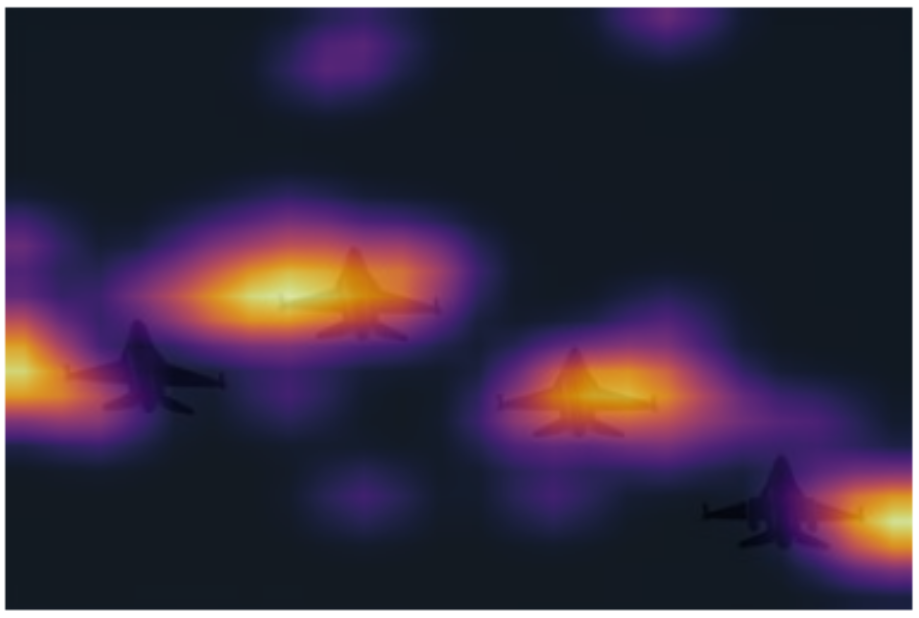
\includegraphics[width=0.8\linewidth]{figures/planes_attn.png}
    \caption{Attention saliency when the model is asked to count four planes.}
    \label{fig:planes_attn}
\end{figure}

\textbf{Raw gradients} behaved oppositely: broadly distributed, with high scores on many tokens. In useful cases two regimes appeared: either the gradients fully covered the region of interest, or they concentrated entirely on irrelevant areas, the inverse of the correct map. Our maps suggest, though do not confirm, that the first regime coincides with correct predictions and the second with incorrect ones. We also observed no visual correspondence between a layer's attention map and its gradient map.

\textbf{CAM variants} mix attention and gradients with simple transforms (e.g., ReLU). These were hit-or-miss: when they worked they produced maps that cleanly covered the objects of interest, but roughly a quarter of the time they were less interpretable than either ingredient. AGCAM (which additionally applies a sigmoid to the attention) produced the best maps when it worked but was less consistent than the more reliably interpretable GradCAM. We see room for a CAM variant tuned specifically to VLMs.

\textbf{Layers and heads.} Early-layer attention maps were far more interpretable than late-layer ones, where contextualized tokens attend less to the image. We saw strong evidence for localization heads~\citep{kang2025your} (a few heads do most of the looking and yield the cleanest maps), though the spatial-entropy heuristic for finding them was only mediocre.

\textbf{Aggregation and transforms.} Among aggregation rules, mean, max, and sum worked best, in that order; individual heads were complementary, each attending where others did not. Binarization and Gaussian smoothing both improved interpretability.

\begin{figure}[t]
    \centering
    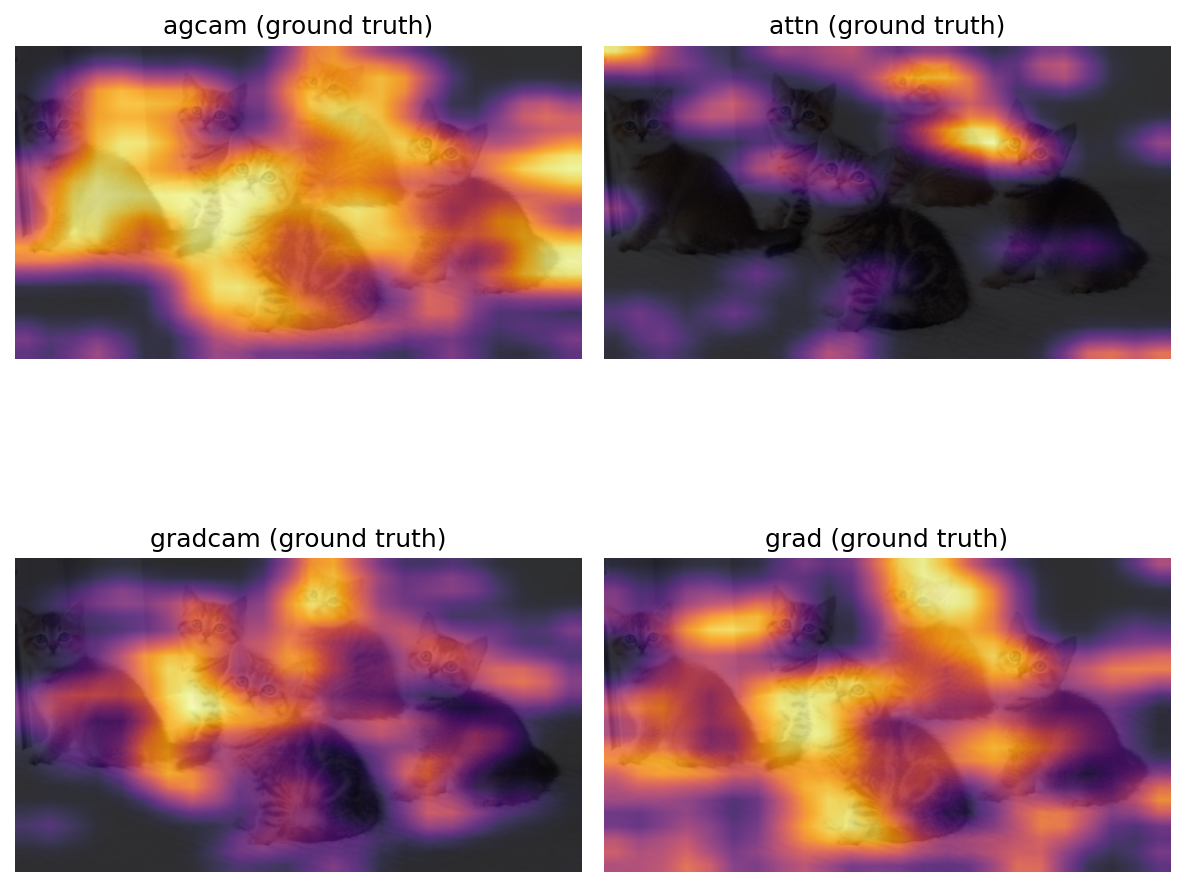
\includegraphics[width=0.8\linewidth]{figures/fourcats.png}
    \caption{The four attribution methods for the token ``four'' in the prompt \emph{``How many cats are in the image? There are four cats.''}}
    \label{fig:fourcats}
\end{figure}


\section{Saliency and Counting}
\label{app:counting}
Counting motivated much of this work, and we report here two negative results that shaped our focus on direct attention supervision.

Counting is deceptively hard for VLMs: they must map visual features to a discrete numeral with no explicit enumeration mechanism. We observe that saliency maps localize cleanly to the relevant objects only when the count is small---typically fewer than five---suggesting that current models lean on holistic pattern recognition rather than individuated object identification as counts grow.

\textbf{Count-specific fine-tuning does not sharpen saliency.} Contrary to results on unimodal vision transformers, where count supervision sharpens attention toward the relevant regions~\citep{paiss2023teachingclipcount}, we find this does not transfer to VLMs. Fine-tuning LLaVA-1.5-7B and Gemma~3~4B on PixMo-Count~\citep{deitke2024molmopixmoopenweights} improved counting accuracy by roughly $10\%$ but left saliency localization unchanged---accuracy and grounding moved independently.

\textbf{Saliency overlap does not predict counting accuracy.} We tested whether a model's internal spatial focus tracks its counting accuracy, as it would if counting were grounded rather than purely linguistic. Extracting saliency under several attribution methods and measuring its overlap with ground-truth object masks on a COCO-derived subset of TallyQA~\citep{acharya2019tallyqa}, we found that saliency mass inside the annotated regions does \emph{not} correlate with correct counts.

Together these results say that counting accuracy and attention localization are decoupled under the standard objective: improving the answer does not improve the looking, and \emph{vice versa}. This is precisely what motivates supervising localization directly, as in the main paper, rather than hoping it emerges from a task loss.


\section{Saliency Hallucination}
\label{app:hallucination}
A final observation concerns how saliency behaves for \emph{incorrect} predictions. When a VLM miscounts---answering ``four'' for an image of three cats---we often (though not always) see a phantom blob of attention in the background, structurally similar to the mass on the three real objects, as if the model attends to evidence for an object that is not there. The complementary error also occurs: when the model undercounts (``two'' for three cats), the saliency skips the missed object entirely. The effect was visible in somewhat more than half the images we examined, most clearly for large objects and small counts. We report it as a qualitative phenomenon; quantifying this ``saliency hallucination'' and relating it to answer errors is an interesting direction we did not pursue here.


\end{document}


% This document was modified from the file originally made available by
% Pat Langley and Andrea Danyluk for ICML-2K. This version was created
% by Iain Murray in 2018, and modified by Alexandre Bouchard in
% 2019 and 2021 and by Csaba Szepesvari, Gang Niu and Sivan Sabato in 2022.
% Modified again in 2023 and 2024 by Sivan Sabato and Jonathan Scarlett.
% Previous contributors include Dan Roy, Lise Getoor and Tobias
% Scheffer, which was slightly modified from the 2010 version by
% Thorsten Joachims & Johannes Fuernkranz, slightly modified from the
% 2009 version by Kiri Wagstaff and Sam Roweis's 2008 version, which is
% slightly modified from Prasad Tadepalli's 2007 version which is a
% lightly changed version of the previous year's version by Andrew
% Moore, which was in turn edited from those of Kristian Kersting and
% Codrina Lauth. Alex Smola contributed to the algorithmic style files.
